%
%  outline latex source document for AILP assignment 3.
%  use pdflatex to format this (and bibtex if use external bibliography)
%
\documentclass[10pt,a4paper,twocolumn]{article}
\usepackage{amssymb,amsmath}            % if some maths is needed
\usepackage{graphicx}                   % if any images are to be included
% pick a different font if desired
\usepackage{times}

\usepackage{listings}
\usepackage{color}
\usepackage{hyperref}

\definecolor{dkgreen}{rgb}{0,0.6,0}
\definecolor{gray}{rgb}{0.5,0.5,0.5}
\definecolor{mauve}{rgb}{0.58,0,0.82}

\lstset{frame=tb,
  language=XML,
  morekeywords={Argument, name, proof, premises, exceptions, weights,
  conclusion, truth, negate, weight, assumptions, CMLObject, Proposition,
  MarkupObject, attributeOfObject, MarkupObject, anotherAttributeOfObject,
  CMLAttribute, CMLAttribute1, CMLAttribute2, CMLAttribute3, CAES,
  CMLAttribute3},
  morecomment=[s]{<!}{!>},
  aboveskip=3mm,
  belowskip=3mm,
  showstringspaces=false,
  columns=flexible,
  basicstyle={\small\ttfamily},
  numbers=none,
  numberstyle=\tiny\color{gray},
  keywordstyle=\color{blue},
  commentstyle=\color{dkgreen},
  stringstyle=\color{mauve},
  breaklines=true,
  breakatwhitespace=true,
  tabsize=3
}

\title{AILP (2016) Report}               % AILP: please use this title.
\author{by Levi Fussell (s1408726)}      
\date{1st December 2016}                 % replace with actual date

\begin{document}

\maketitle  % this inserts title, author info
%
\section{Introduction}

The following report describes work done in the AILP
course over the course of three months. It gives the aims and hypothesis that guided the work;
describes the algorithms that were implemented; reports the results
of experiments that were run; and analyses these results.

\section{Aim}

This assignment was designed as a gentle introduction to the concept of argumentation systems,
and the different features that must be considered when implementing a full
argumentation system.

\section{What is an argumentation system?}

As all who have
once been a child whinging and shouting at their parents would know, arguing has
a varied audience and an immeasurable history. We argue daily
with others concerning clothing prices and opinions and we argue internally with our
emotions and whether we should ask that girl out. The concept of argumentation merely attempts to
formalise and make sensible this constantly bickering world we live in.

An argument is composed of three major pieces: its premises, its conclusion,
and an inference from the premises to conclusion \cite{ES2}. Each of
these pieces is represented by propositions, an atomic statement that is either
true or false. A system of arguments composes related arguments into an
organised manner. Generally, we represent this as an argument tree.
Arguments form chains where the conclusion of one argument is the premise for
another argument, and vice versa. Arguing is akin to the 80s Tron Sinclair game:
each party rides a bike that generates a longer and longer tail - the
challenge is to keep your bike (argument) alive by craftily averting your
oponent's tail, yet
simultaneously aiming to fatally catch your opponent off guard with your tail.

\begin{figure}[h]
  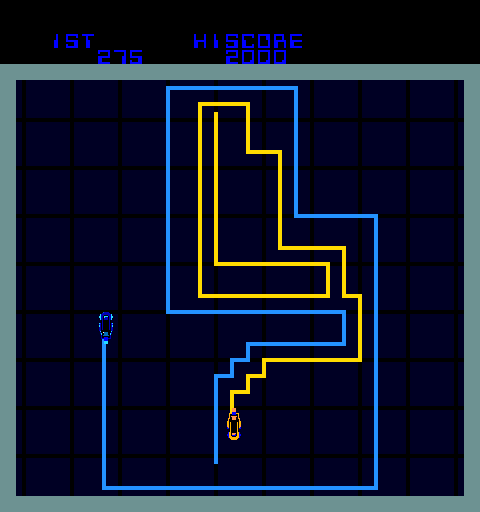
\includegraphics[width=6cm]
  {images/lightCycle.png}
  \centering
  \caption{Old videogames still have their use when it comes to analogies.
	  \href{http://www.arcade-history.com/images/game/2979_1.png }{source}}
\end{figure}

The light tail of our bike in an argumentation context is driven by sequentially declaring
more arguments in favour of your position. The opposing party drives their tail
through invoking new arguments, or disproving your previous arguments. If
a party has no more arguments to support their case, game over - they have
smashed into their opponent's light tail.

In an argumentation system, we are hoping to automate the oscillating behaviour
of arguing. The system has many complex decisions and weighing of options it has
to perform, such as whether to raise a critical question to undermine an
opponent's earlier argument, or affirm their current position by bringing to light an
argument with grounded assumptions/evidence.

\section{What is Carneades?}

Inventing the AI that would solve all arguments in all domains would be a feat.
Sadly, this is fanciful talk, but a particular area has seen
much advancement concerning AI and argumentation: law. Carneades is an
argumentation framework designed for dialogue arguments between two parties and
is designed specifically with the use of law cases in mind. Unlike the
traditional definition of an argument, Carneades represents an argument with different types of
premises that pose critical questions about the argument. The three types
are exceptions, wherein if any exception is proven true, the argument cannot
stand, assumptions, which are assumed true by the audience (as in evidence), and
premises, which all must be true or assumed, in order for the argument to hold
\cite{ES4}.

Carneades implements a burden of proof model. The burden of proof is on
whichever party, based on all current arguments and assumptions thus far, has to present the
next argument to avoid losing. Arguments are continuously presented by the party with the
burden of proof until the proposition that both parties are arguing has been
accepted or rejected in favour of one party. Propositions are accepted in
a recursive manner depending on the defensibility of the pro and con arguments
for that proposition.
An argument is defensible if its premises hold and its exceptions do not hold.
To determine the truth of the argument's premises we must begin the cycle again at choosing
arguments \cite{ES4}. Hence, the
argument proof descends down the argumentation tree.

\section{Algorithms and implementation}

For this purpose the following extensions were carried out
\begin{enumerate}
\item reading of input from text files
\item making the system capable of dynamically constructing arguments and
	determining the burden of proof between two
	parties
\end{enumerate}

\subsection{extending the system to read from text files}

Extending the system to read from text files was not only to allow the less
program-orientated users to implement an argumentation scheme, but also to
simplify the system so that arguments could quickly be analysed. The Carneades
python framework required the user to pre-define propositions, create an
argument set, and create an audience before the arguments could be analysed. The
goal of the text file reading is to remove those trivialities.

The \textit{Carneades Markup Language} is a basic markup language that is used 
to simplify the compiling of Carneades Python programs. It imitates a 
simplified version of basic markup:

\begin{lstlisting}
<MarkupObject>
  <attributeOfObject>
  big
  </attributeOfObject>
  <anotherAttributeOfObject>
  200
  </anotherAttributeOfObject>
</MarkupObject>

<!> This is a one line comment <!>
\end{lstlisting}


The simplified markup implementation uses only two layers of markup to describe different Carneades classes. The highest order line,

\begin{lstlisting}
<CMLObject>...</CMLObject>
\end{lstlisting}

represents the definition of a Carneades class. The only available Carneades classes in CML are:

\begin{lstlisting}
<Proposition>...</Proposition>
<Argument>...</Argument>
<CAES>...</CAES>
\end{lstlisting}

(NOTE: classes not implemented, such as \textit{ProofStandard, Audience, ArgumentSet}, 
are all created at compile-time; this design decision will be discussed later)

Each Carneades class has a series of CML \textit{attributes} that are used to define 
unique details about a specific object. Without these \textit{attributes} 
implemented, the generic classes will fail. It is important to note that 
the order in which \textit{attributes} are written does not matter, but only 
some \textit{attributes} can be excluded (similar to the concept of a const
ructor). An \textit{attribute} is defined as a markup object that is one mark
up layer inside a markup \textit{class} object (which is always at layer zero) 
and has a \textit{value item} one layer inside it:

\begin{lstlisting}
<CMLObject>
  <CMLAttribute>
  value\_of\_attribute
  </CMLAttribute>
</CMLObject>
\end{lstlisting}

The inclusion of the \textit{value item} (value\_of\_attribute\_) is required for the obje
ct to be an \textit{attribute}. The name of the value, class objects and attribute object
s follow the general naming scheme of python variables. \textit{Attributes} are written in series:

\begin{lstlisting}
<CMLObject>
  <CMLAttribute1>
  value\_of\_attribute1
  </CMLAttribute1>
  <CMLAttribute2>
  value\_of\_attribute2
  </CMLAttribute2>
</CMLObject>
\end{lstlisting}

Order (as well as spacing) is irrelevant:

\begin{lstlisting}
<CMLObject>

  <CMLAttribute2> value\_of\_attribute2 </CMLAttribute2>

  <CMLAttribute3> <!> comment about this attribute, etc... <!>
    value\_of\_attribute3
  </CMLAttribute3>

  <CMLAttribute1>value\_of\_attribute1
  </CMLAttribute1> </CMLObject>
\end{lstlisting}

The \textit{class/attribute} combinations (constructors) for each class are displaye
d below. Optional \textit{attributes} are indicated by a comment:

\begin{lstlisting}
<!>PROPOSITIONS<!>
<Proposition>
  <name>...name ID of proposition...</name>
  <truth>...truth value of the proposition. Default value is 'True'...</truth> <!>optional<!>
  <proof>...standard of proof for the proposition. Default value is 'scintilla'...</proof> <!>optional<!>
</Proposition>

<Proposition>
  <name>...name ID of proposition...</name>
  <negate>...name-tag of the proposition to copy and negate...</negate>
  <proof>...standard of proof for the proposition. Default value is 'scintilla'...</proof> <!>optional<!>
</Proposition>

<!>ARGUMENTS<!>
<Argument>
  <name>...name ID of argument...</name>
  <conclusion>...conclusional proposition of the argument...</conclusion>
  <premises>...[list, of, premises, of, the, argument]...</premises>
  <exceptions>...[list, of, exceptions, of, the, argument]...</exceptions> <!>optional<!>
  <weight>...float value of the weight of this argument...</weight>
</Argument>

<!>CAES<!>
<CAES>
  <name>...name ID of CAES...</name>
  <assumptions>[list, of, propositions, that, are, audience, assumptions]</assumptions>
</CAES>
\end{lstlisting}

Some syntactical notes:
\begin{itemize}
	\item {There are 6 types of attributes of which 4 are used when writing CML in a text file:
		\begin{enumerate}
		  \item \textit{String}: any attribute that has written text (make sure to exclude '...', unlike other languages)
		  \item \textit{Number}: any attribute that has only a float value (i.e. 0.6)
		  \item \textit{Bool}: any attribute that contains the word true/false with any capitalisation. This overrides a string type
		  \item \textit{StringList}: any attribute that starts and ends with '[...]' and contains comma-seperated strings
		\end{enumerate}}
	\item {(IMPORTANT) Defining each proposition before the arguments is not strictly necessary. 
	Arguments will intuitively add propositions that are missing from implementation (
	this will not happen with the \textit{CAES assumptions attribute}, these propositions 
	must be predefined in an argument/proposition. It is important to note that this implementation 
	can be dangerous; miss-spelt proposition names will be treated as \textit{new} propositions. 
	Be careful!). There are a few special cases:
	\begin{enumerate}
		\item If the \textit{proof} value of a proposition needs to be set to a value other than the default value, 'scintilla', then a proposition must be predefined before the argument(s).
		\item If a \textit{negated} proposition needs to be implemented, this can be done by adding the exact string 'neg\_' to the start of the proposition's name, like so:
	\end{enumerate}}
\end{itemize}
\begin{lstlisting}
\dot
<premises>\dot[prop2, neg\_prop3]\dot</premises>
\dot
\end{lstlisting}

(NOTE: neg\_prop3 will make 2 propositions if prop3 has not been defined earlier: prop3 and -prop3)

\subsection{extending the system to argue}

The system now has the capability to take a set of arguments along with an audience and
determine whether a proposition is applicable using the generated argument tree.
A useful feature to this system would be the ability to observe how the various
arguments are used by both the prosecution and the defense to form the final
conclusion.

We start by thinking about how the simplest argument system would function. This
involves discussing where the burden of proof (as defined earlier) lies within an argumentation
system. The goal of each party in an argument is to shift the burden of proof
away from themselves and onto their opponent and, further, make it harder for
the opponent to shift the burden of proof back onto the original party. To
shift the burden of proof the party therefore has two goals: find some
argument(s) sequence that will shift the burden of proof, and find the
argument(s) sequence that is the strongest (this prevents the burden of proof
from shifting back to the original party). 

In a simple scenario, where we assume a single argument shifts the burden of
proof, an argument can either prove the conclusion the parties are fighting for
in favour of the burdened party, undermine an argument that the opposing party
has made, or build from a previous weak argument that the current party has
made. As an argument system progresses and each argument is posed by a party, we
need to keep track of the weak propositions within each argument. Weak
propositions are those that are not in the audience assumptions and do not have
any arguments for/against them. As shown below:

\begin{figure}[h]
  \includegraphics[width=6cm]
  {images/ArgumentSearchSim.png}
  \centering
  \caption{(green=target argument proposition, red=current weak
  propositions)}

\end{figure}

If an argument is posed and its premises contain
a weak proposition, that argument is not applicable. Alternately, weak
propositions are routes of attack for a party. When the burden of proof
alternates, so do the polarities of the weak propositions; the new party can
therefore attack the weak propositions and undermine the opposing party's
argument(s). When the party with the burden is arguing, its goal is to pose
arguments until the proposition both parties are arguing over is acceptable
given the current
assumptions and already posed arguments. A good heuristic for determining which
arguments to choose is to select arguments which prove any of the weak
propositions.

At the beginning of an argument between two parties, the only weak
proposition is the proposition the two parties are arguing for (e.g. was it murder,
getting a fine/ticket, etc.) and therefore the first party's most sensible move is to
pose an argument for that proposition. Because the list of possible arguments
could be vast, a heuristic graph-search algorithm is introduced. The weak propositions
are added to a list and the current party's choice for a weak proposition
to target with an argument is the best choice best on some heuristic measure.
Different heuristic choices and graph algorithms were experimented with in Table
1 \ref{table1}.

Once a path has been chosen that results in the
proposition the two parties are arguing for being acceptable (in the case of the defense) or not
acceptable (in the case of the prosecution), the full argument sequence is
composed by traversing the assembled graph via the chosen arguments back to the start.
The Burden of Proof then changes hands. We can see this process in the argument
simulation in the figure \ref{simOfHeuristics}:

\begin{figure}[h!]
	\label{simOfHeuristics}
	\includegraphics[width=6cm]{images/ArgumentSearchSim2-2.png}
	\centering
	\caption{simulation of depth-first searching the argument graph}
\end{figure}

A brief statement on how the burden of proof system is displayed when running
the program. When the test case is selected and run, the argument system will go
through a sequence of steps. Each step either describes how the party with the
burden of proof is searching for an effective argument sequence (and describes
the most recent argument that has been searched):

\begin{figure}[h!]
	\label{screen1}
	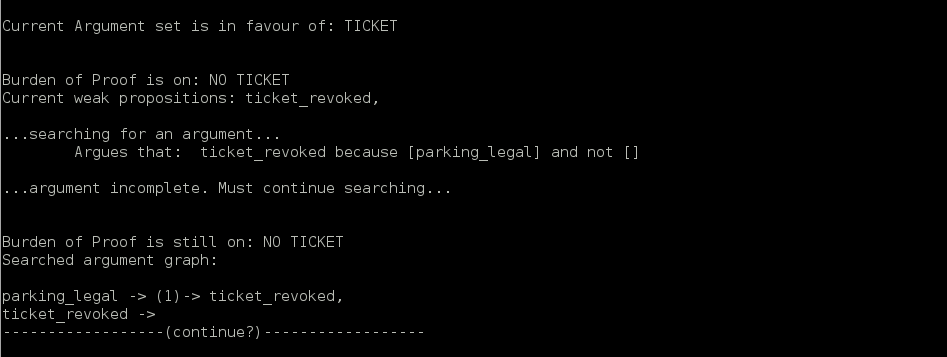
\includegraphics[width=6cm]{images/screeen1.png}
	\centering
	\caption{Current party is searching for an argument.}
\end{figure}

Or describes how the current party has succeeded in finding an effective
argument sequence (additionally it will display the sequence of propositions in the graph
that derive the argument chain).

\begin{figure}[h!]
	\label{screen2}
	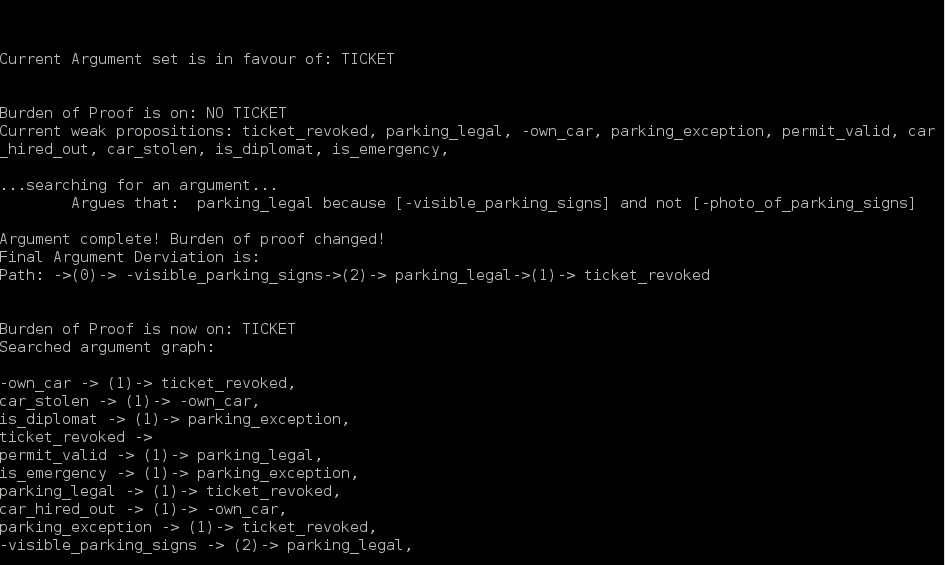
\includegraphics[width=6cm]{images/screeen2.png}
	\centering
	\caption{Current party has found an argument.}
\end{figure}

If all arguments have been exhausted and the current party is unable to change
the burden of proof, then the current party has lost the argument. The opposing
party is deemed the 'winner'. Note that 'Prosecution' and 'Defense' are renamed
to names more relevant to each test case so that the system can be understood.
The end of each step outlines the current situation of the argument graph using
an inverted-index format.

A good demonstration of the burden of proof changing hands multiple times is in
test case '2' (when running 'main.py')

\section{Experiments and results}

\subsection{experimenting with the argumentation heuristics}
How different hueristic algorithms applied to the argumentation search affected
the speed of determining the next argument sequence, and also whether the
argument sequence determined was the most optimal.

\begin{table} [t,h!]
	\caption{\label{table1} Experimenting with different graph searching
	algorithms.}
	\vspace{1mm}
	\centerline{
		\begin{tabular}{|c|c|c|c|}
			\hline
			algorithm & branch order & itteration & best solution? \\
			\hline  \hline
			depth-first search & B1,B2,B3,B4 & 6 & no\\
			depth-first search & B4,B3,B2,B1 & 3 & yes\\
			depth-first search & B1,B4,B3,B2 & 2 & yes\\
			depth-first search & B2,B4,B1,B3 & 4 & no\\
			depth-first search & B2,B3,B1,B4 & 7 & no\\
			\hline
			breadth-first search & B2,B3,B1,B4 & 5 & yes\\
			breadth-first search & B4,B3,B2,B1 & 7 & yes\\
			breadth-first search & B1,B4,B3,B2 & 7 & yes\\
			breadth-first search & B2,B4,B1,B3 & 5 & yes\\
			breadth-first search & B2,B3,B1,B4 & 5 & yes\\
			\hline
			min-weight-first search & B2,B3,B1,B4 & 5 & no\\
			min-weight-first search & B4,B3,B2,B1 & 5 & no\\
			min-weight-first search & B1,B4,B3,B2 & 5 & no\\
			min-weight-first search & B2,B4,B1,B3 & 5 & no\\
			min-weight-first search & B2,B3,B1,B4 & 5 & no\\
			\hline
			djikstra search & B2,B3,B1,B4 & 6 & yes\\
			djikstra search & B4,B3,B2,B1 & 6 & yes\\
			djikstra search & B1,B4,B3,B2 & 6 & yes\\
			djikstra search & B2,B4,B1,B3 & 6 & yes\\
			djikstra search & B2,B3,B1,B4 & 6 & yes\\
			\hline
		\end{tabular}
	}
\end{table}

\begin{table} [t,h!]
	\caption{\label{table2} Averaged results of different graph searching
	algorithms.}
	\vspace{2mm}
	\centerline{
		\begin{tabular}{|c|c|c|}
			\hline
			algorithm & avg itterations & accuracy\\
			\hline  \hline
			depth-first search & 4.4 & 2/5\\
			\hline
			breadth-first search & 5.8 & 5/5\\
			\hline
			min-weight-first search & 5 & 0/5\\
			\hline
			djikstra search & 6 & 5/5\\
			\hline
		\end{tabular}
	}
\end{table}

\clearpage{}

\section{Discussion and Conclusion}

\subsection{analysis of experiments}
Experimenting with different heuristic graph searches posed some interesting
results. This data was collected via the following simulated test case:

\begin{figure}[h!]
	\label{ArgumentHeuristics}
	\includegraphics[width=8cm]{images/ArgumentHeuristics.png}
	\centering
	\caption{Test case used to measure heuristics algorithms. Weight of each
	argument given by 'w'. 'B\#' is the name of each branch. These are shuffled
	in different orders at testing time. Only branch 'B2' and 'B3' produce an
argument sequence that makes 'T0' applicable.}
\end{figure}
This can be run by selecting option '4' at the start of the 'main.py'
program and then selecting which heuristic you would like to run for selecting
arguments. The weights between two arguments are determined by how weak that
argument is. A higher weight corresponds to a higher weakness. Weakness of an
argument is the sum of its premises and exceptions. This is a sensible choice
because arguments that are more 'complex', i.e. have more propositions to
prove/disprove it, are more likely to be defeated by the opposition. The current
holder of the burden of proof therefore favours simpler arguments that are
easier to prove and harder to be defeated.

From the final data, the best performing heuristics were
breadth-first search and djikstra (as hypothesised, considering djikstra is one of
the most commonly used heuristics). Both algorithms found the
best solution each time. Although the breadth-first search had the lowest
average number of iterations, the test graph was an exclusive case where
the best solution was always at a higher depth than other solutions, therefore
breadth-first search would always select the best solution. Breadth-first search
also had a much higher variance when it came to number of iterations.
Djikstra is therefore left as the best option for traversing the
argument graph due to its consistency and ability to always find the strongest
argument.
\subsection{how this system could be extended further}
One topic that would have been beneficial to explore further would be how the weights
are assigned to different arguments for the graph search. The current method of
using the total number of premises and exceptions was an arbitrary choice based
on a general concept of how arguments can be deemed strong or weak. Weights
based on the depth of the argument in the tree, weights based on the probability of a chosen
proposition leading to an assumption, and also larger trees to search would have
allowed for an interesting analysis of the argumentation system and the extents
to which it can perform in more realistic scenarios. Overall, it is quite
impressive how a relatively simple system can perform such a convincing display
of argumentation. Given the hardest piece to the argumentation system is the
construction of an affective argumentation graph, there is definite room for
further complexity and interesting evolutions of how to traverse this graph.

%
\bibliographystyle{plain}
\bibliography{ailp_latex_biblio.bib}
\end{document}

%%% Local Variables:
%%% mode: latex
%%% TeX-master: t
%%% End:
